\documentclass{article}
\usepackage[a4paper, total={7in, 10in}]{geometry}
\usepackage{stmaryrd}
\usepackage{amssymb}
\usepackage{amsmath}
\usepackage{amsthm}
\usepackage[french]{babel}
\usepackage{tcolorbox}
\usepackage{graphicx}
\begin{document}
\begin{flushleft}

\author{José Lorgeré}

\title{TIPE - Connexité et lacets à intersection dans le plan}

\maketitle

\begin{abstract}
    Le théorème de Jordan est un théorème phare en topologie, connu notamment pour son énoncé intuitif, contrastant avec les
    outils nécessaires pour aboutir à une démonstration de ce dernier. Dans ce TIPE, on définit formellement la notion d'autointersection
    pour des chemins, et on aboutit à un théorème généralisant celui de Jordan, permettant de quantifier le nombre de composantes
    connexe par arcss du complémentaire dans le plan de certains lacets
\end{abstract}

\section{Définitions usuelles et notations}

Dans tout le document, on notera $\sqcup$ les unions disjointes\\
\begin{tcolorbox}[colback = yellow!60!white, colframe = orange!90!white, title = Définition]
    Un chemin de $x$ à $y$ est une application $\gamma : [0, 1] \longrightarrow \mathbb{R}^2$ continue telle que $\gamma(0) = x$ et $\gamma(1) = y$
\end{tcolorbox}
\vspace{0.5cm}
Si $\gamma$ est un chemin, on dénotera également son image par $\gamma$ 
\begin{tcolorbox}[colback = yellow!60!white, colframe = orange!90!white, title = Définition]
    Un lacet est un chemin $\gamma$ tel que $\gamma(0) = \gamma(1)$
\end{tcolorbox}
\vspace{0.5cm}
\begin{tcolorbox}[colback = yellow!60!white, colframe = orange!90!white, title = Définition]
    Une courbe de Jordan est un lacet injectif sur $[0, 1[$
\end{tcolorbox}
Le théorème de Jordan s'énonce alors comme
\begin{tcolorbox}[colback = purple!20!white, colframe = purple!60!white, title = Théorème de Jordan]
Soit $\gamma$ une courbe de Jordan\\
Alors $\mathbb{R}^2 \backslash \gamma$ a deux composantes connexes par arcs ouvertes, l'une bornée, l'autre non, ayant toutes deux pour
frontière $\gamma$
\end{tcolorbox}
\vspace{0.5cm}
Le théorème suivant vient compléter l'information donnée par le théorème de Jordan
\begin{tcolorbox}[colback = purple!20!white, colframe = purple!60!white, title = Théorème de Jordan-Schönflies]
    Soit $\gamma$ une courbe de Jordan\\
    Notons $V$ sa composante bornée\\
    Il existe un homéomorphisme de $\mathbb{R}^2$ dans lui même, tel que l'image de $V$ par ce dernier
    soit $\mathcal{B}(0, 1)$ et celle de $\gamma$ soit $\mathcal{S}(0, 1)$
\end{tcolorbox}
\vspace{0.5cm}

\begin{figure}[h]
    \caption{Illustration du théorème de Jordan}
    \centering
    La zone en rouge est la composante non bornée, celle en bleu la bornée\\
    \vspace*{0.2cm}
    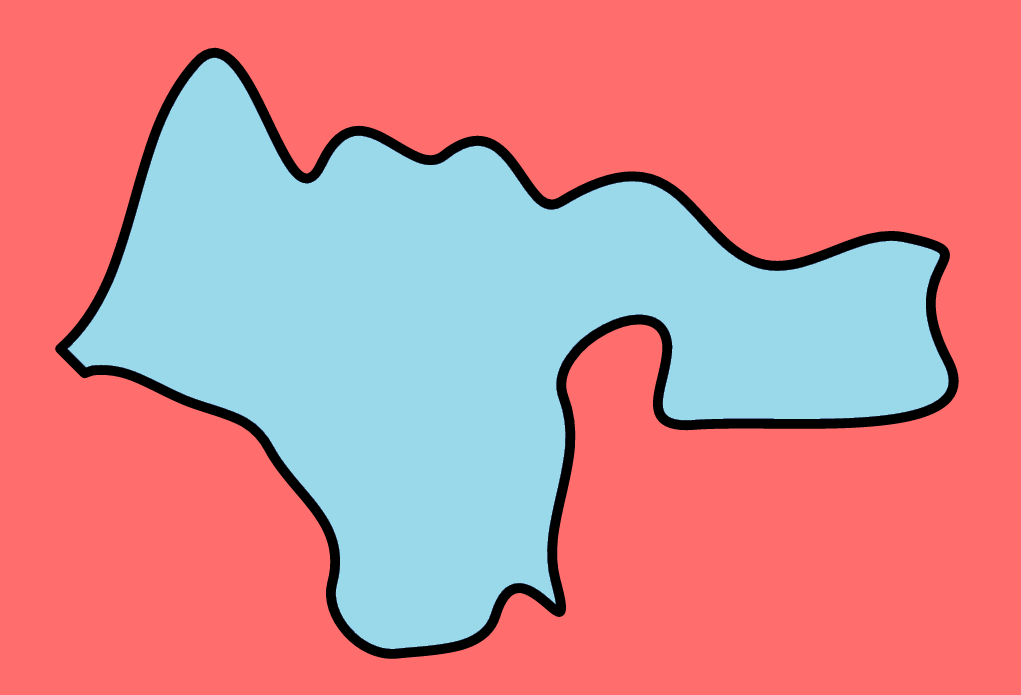
\includegraphics[width = 0.6 \textwidth]{Jordan.png}

\end{figure}

Ces résultats portant uniquement sur des courbes de Jordan, on se demande alors : que se passerait-il si on affaiblissait
l'hypothèse d'injectivité ? 

\section{Problème}

On va ici développer des outils pour quantifier à quel point un lacet "s'autointersecte", et définir un ensemble de lacets particuliers
\\~\\
\begin{tcolorbox}[colback = yellow!60!white, colframe = orange!90!white, title = Définition 1]
    Soit $\gamma$ un chemin\\
    On note
    \[I_{\gamma} = \{ x \in \gamma \mid \exists t_1 \neq t_2 \in [0, 1], x = \gamma(t_1) = \gamma(t_2) \}\]
    l'ensemble des intersections de $\gamma$
\end{tcolorbox}
\vspace{0.5cm}
\begin{tcolorbox}[colback = yellow!60!white, colframe = orange!90!white, title = Définition 2]
    Soit $x \in I_{\gamma}$\\
    Si $\gamma^{-1}(\{x\})$ est fini, on note $S(x)$ le "nombre de sorties" de $x$ l'entier suivant
    \[S(x) = |\gamma^{-1}(\{x\})|\]
\end{tcolorbox}
\vspace{0.5cm}
\begin{tcolorbox}[colback = yellow!60!white, colframe = orange!90!white, title = Définition 3]
    Soit $\gamma$ un chemin\\
    Si $I_{\gamma}$ est fini et pour tout $x \in I_{\gamma}$, $S(x)$ est défini, on dira que $\gamma$ est à retours finis
    et on note le nombre de retours
    \[r(\gamma) = \sum_{x \in I_{\gamma}} (S(x) - 1)\]
\end{tcolorbox}

Notons que selon ces définitions, $\gamma(0)$, le point ou le lacet se referme, compte comme une intersection, donc $\gamma(0) \in I_{\gamma}$\\
Le nombre de lacets du lacet Figure 2 est alors de 4\\

\begin{figure}[h]
    \caption{Un exemple de lacet à retours finis}
    \centering
    Le point noir représente $\gamma(0)$\\
    \includegraphics*[width=0.5\textwidth]{Lacet retours finis.png}
\end{figure}

Notons que le lacet Figure 2 délimite 4 composantes connexes par arc bornées\\
On cherchera alors à montrer le théorème suivant
\begin{tcolorbox}[colback = purple!20!white, colframe = purple!60!white, title = Théorème des retours]
    Soit $\gamma$ un lacet à retours finis\\
    $\gamma$ délimite $r(\gamma)$ composantes connexes par arcs bornées
\end{tcolorbox}

L'idée générale de la démonstration sera basée sur le constat suivant : lorsque l'on trace le lacet, à la main par exemple, chaque fois
que le nombre de retours augmente, une nouvelle composante connexe par arcs est créée. On formalisera par la suite ce constat

\section{Connexité par arcs dans le plan}

Avant de démontrer le théorème, on se dote d'abord de quelques propriétés utiles des connexes par arc de $\mathbb{R}^2$

\subsection{Une géneralisation des valeurs intermédiaires}

\begin{tcolorbox}[colback = purple!20!white, colframe = purple!60!white, title = Proposition 1]
    Soit $A$ un connexe par arcs et $B \subset \mathbb{R}^2$ tel que $A \cap B \neq \varnothing$
    et $A \backslash B \neq \varnothing$\\
    Alors $A \cap \operatorname{Fr}(B) \neq \varnothing$
\end{tcolorbox}

\begin{proof}
Soient $x \in A \backslash B$, $y \in A \cap B$\\
Soit $c$ un chemin de $x$ à $y$ dans $A$ par connexité par arcs\\
Donc $c(0) \in A \backslash B$, on peut alors considérer
\begin{equation*}
    t_0 = \sup \{ t \in [0, 1] \mid c(t) \in A \backslash B \}
\end{equation*}
Si $t_0 \neq 0$ et $t_0 \neq 1$ :\\
Alors :
\begin{equation}
    \forall s \in ]0, t_0[, \exists t \in ]s, t_0[,
c(t) \in A \backslash B
\end{equation}
et
\begin{equation}
\forall t \in ]t_0, 1[, c(t) \in A \cap B
\end{equation}
Par continuité de $c$ et (2) et (3) toute boule ouverte centrée en $c(t_0)$ rencontre $A \cap B$ et $A \backslash B$\\
On obtient alors que $c(t_0) \in \operatorname{Fr}(A \cap B) \subset \operatorname{Fr}(B)$
\\~\\
Si $t_0 = 0$, on a juste (3) et le fait que toute boule centrée en $c(0)$
contient $c(0)$ et rencontre donc $A \backslash B$.\\
On aboutit alors au même résultat\\
Si $t_0 = 1$ même chose, mais avec (2)

\end{proof}

\subsection{Composantes connexes par arcs d'un ouvert}

\begin{tcolorbox}[colback = purple!20!white, colframe = purple!60!white, title = Proposition 2]
    Soit $V$ un ouvert\\
    Ses composantes connexes par arcs sont ouvertes
\end{tcolorbox}

\begin{proof}
    Si $V$ est connexe par arcs, on a déjà le résultat
    \\~\\
    Si $V$ ne l'est pas, notons $\mathcal{C}$ l'ensemble de ses composantes et prenons $U \in \mathcal{C}$\\
    Supposons par l'absurde que $U$ n'est pas ouvert, soit $U \cap \operatorname{Fr}(U) \neq \varnothing$\\
    Soit $x \in U \cap \operatorname{Fr}(U)$\\
    Comme $U \subset V$, il existe $r > 0$ tel que $\mathcal{B}(x, r) \subset V$, et on a également comme
    $\mathcal{B}(x, r) \backslash U \neq \varnothing$\\
    Comme
    \[ V = \bigcup_{U' \in \mathcal{C}} U' \]
    il existe donc $U' \in \mathcal{C} \backslash \{U \}$ tel que $\mathcal{B}(x, r) \cap U' \neq \varnothing$\\
    $\mathcal{B}(x, r)$ étant connexe par arcs inclus dans $V$ et rencontrant $U$ et $U'$, il existe un chemin dans
    $V$ de $U$ à $U'$, ce qui est absurde car ces deux composantes connexes par arcs sont distinctes
    \\~\\
    Donc $U$ est ouvert
\end{proof}
\vspace*{0.5cm}

Après cette proposition, on considèrera que toutes les composantes connexes par arc manipulées seront des ouverts
\\~\\
\begin{tcolorbox}[colback = purple!20!white, colframe = purple!60!white, title = Proposition 3]
    Soit $U$ un ouvert et $(V_i)_{i \in I}$ ses composantes connexes par arc\\
    On a
    \[ \bigcup_{i \in I} \operatorname{Fr}(V_i) \subset \operatorname{Fr}(U) \]
    On a l'égalité si $I$ est fini
\end{tcolorbox}

\begin{proof}
    Soit $i \neq j \in I$\\
    Notons que $\overline{V_i} \subset \mathbb{R}^2 \backslash V_j$\\
    En effet, si ce n'était pas le cas, il existerait un point dans $\overline{V_i}$ et $V_j$\\
    $V_j$ est un voisinage de ce point, étant un ouvert, et ainsi rencontre $V_i$\\
    Or ce sont des composantes distinctes, ce qui justifie l'inclusion
    \\~\\
    Puis, on a
    \begin{align*}
        \operatorname{Fr}(U) &= \overline{U} \backslash U\\
        &= \left( \overline{\bigsqcup_{i \in I} V_i} \right) \backslash U\\
        &\supset \left( \bigcup_{i \in I} \overline{V_i} \right) \backslash \left( \bigsqcup_{i \in I} V_i \right)\\
        &= \bigcup_{i \in I} \left( \overline{V_i} \bigcap_{j \in I} \mathbb{R}^2 \backslash V_j \right)\\
        &= \bigcup_{i \in I} \overline{V_i} \cap \mathbb{R}^2 \backslash V_i\\
        &= \bigcup_{i \in I} \operatorname{Fr}(V_i)
    \end{align*}
    Si $I$ est fini l'inclusion se transforme en égalité
\end{proof}

\begin{tcolorbox}[colback = purple!20!white, colframe = purple!60!white, title = Proposition 4]
    Soit $U$ un ouvert et $V$ une composante connexe par arcs de $U$\\
    Soit $A$ un connexe par arcs tel que $A \subset U$ et $A \cap V \neq \varnothing$\\
    Alors $A \subset V$
\end{tcolorbox}

\begin{proof}
    Supposons par l'absurde que ce soit faux\\
    Ainsi $A$ rencontre $V$ et son complémentaire\\
    Par connexité et la proposition 1, $A$ rencontre $\operatorname{Fr}(V)$\\
    Par la Proposition 3, $\operatorname{Fr}(V) \subset \operatorname{Fr}(U) \subset \mathbb{R}^2 \backslash U$ car $U$ est ouvert\\
    Donc $A$ rencontre le complémentaire de $U$, absurde par inclusion
    \\~\\
    Donc $A \subset V$
\end{proof}

\begin{tcolorbox}[colback = purple!20!white, colframe = purple!60!white, title = Proposition 5]
    Soit $A \subset \mathbb{R}^2$ tel que
    \[ A = \bigsqcup_{i \in I} V_i \]
    où les $(V_i)_{i \in I}$ sont des ouverts connexes par arcs\\
    Les composantes connexes par arcs de $A$ sont les $(V_i)_{i \in I}$
\end{tcolorbox}

\begin{proof}
    Soit $i \in I$\\
    Comme $A$ s'écrit comme union de ses composantes connexes par arcs, il existe $U$ une composante connexe par arcs de $A$
    tel que $U \cap V_i \neq \varnothing$\\
    Par la Proposition 4, $V_i \subset U$
    \\~\\
    Supposons que $U \neq V_i$, donc $U$ rencontre le complémentaire de $V_i$ dans $A$\\
    Donc $U$ rencontre $\operatorname{Fr}(V_i)$\\
    Donc il existe $x \in A \cap \operatorname{Fr}(V_i)$\\
    Comme $V_i$ est ouvert et par partition, $x \notin V_i$ et donc il existe $j \in I$, $j \neq i$ tel que
    $x \in V_j$\\
    $V_j$ étant ouvert, il s'agit d'un voisinage de $x$\\
    Or tout voisinage de $x$ rencontre $V_i$, donc $V_i \cap V_j \neq \varnothing$, absurde
    \\~\\
    Donc $U = V_i$
\end{proof}

\subsection{Lemme de la ficelle}


\begin{tcolorbox}[colback = purple!20!white, colframe = purple!60!white, title = Lemme]
    Soit $V$ un ouvert borné et $c$ un chemin à valeur dans $\overline{A}$\\
    Pour toute composante connexe par arcs $U$ de $V \backslash c$, on a
    \[ \operatorname{Fr}(U) \cap \operatorname{Fr}(V) \neq \varnothing \text{ et } \operatorname{Fr}(U) \nsubseteq c\]
\end{tcolorbox}

\begin{proof}
    Soit $U$ une telle composante\\
    Supposons par l'absurde que $\operatorname{Fr}(U) \cap \operatorname{Fr}(V) = \varnothing$\\
    On montre dans un premier temps que $\operatorname{Fr}(U) \subset c$
    \\~\\
    Comme $\overline{U} \subset \overline{V}$ et par hypothèse, on a $\operatorname{Fr}(U) \subset V$\\
    Puis, on a par la Proposition 3
    \begin{align*}
        \operatorname{Fr}(U) &\subset \operatorname{Fr}(V \backslash c)\\
        &= \overline{V \cap \mathbb{R}^2 \backslash c} \cap (\mathbb{R}^2 \backslash V \cup c)\\
        &\subset \overline{V} \cap \overline{\mathbb{R}^2 \backslash c} \cap (\mathbb{R}^2 \backslash V \cup c)\\
        &\subset \overline{V} \cap (\mathbb{R}^2 \backslash V \cup c)\\
        &= \operatorname{Fr}(V) \cup (c \cap \overline{V})
    \end{align*}
    Or $\operatorname{Fr}(U) \subset V$, donc $\operatorname{Fr}(U) \subset c \cap \overline{V} \cap V \subset c$
    \\~\\
    Soit $x \in U$. On pose :
    \[ f : \begin{array}{cl}
        \operatorname{Fr}(U) &\longrightarrow \mathcal{S}(0, 1)\\
        u &\longmapsto \frac{u-x}{\|u-x\|}
    \end{array}\]
    $f$ est continue et bien définie car $x \notin \operatorname{Fr}(U)$\\
    Montrons qu'elle est surjective\\
    Soit $v \in \mathcal{S}(0, 1)$\\
    La droite $x + \operatorname{Vect}(v)$ rencontre $U$ et son complémentaire, car $U$ est borné et la droite non\\
    Comme la droite est connexe par arcs, par la Proposition 1, elle recontre $\operatorname{Fr}(U)$ en un point $u$\\
    On a alors que $f(u) = v$\\
    $f$ étant surjective, on se donne $J \subset \operatorname{Fr}(U)$ tel que $f_{\mid J}$ soit une bijection
    \\~\\
    Comme $\operatorname{Fr}(U) \subset c$, il existe $I = c^{-1}(\operatorname{Fr}(U))$ tel que $c_{\mid I}$ soit une bijection continue vers
    $\operatorname{Fr}(U)$\\
    Ainsi, $g = f_{\mid J} \circ c_{\mid I}$ est une bijection continue de $I$ vers $\mathcal{S}(0, 1)$\\
    Soit $\gamma$ une courbe de Jordan surjective dans $\mathcal{S}(0, 1)$\\
    Il existe alors $\Gamma : [0, 1] \rightarrow I$ telle que $g \circ \Gamma = \gamma$\\
    Montrons que $\Gamma$ est continue
    \\~\\
    Supposons qu'il existe $t_0 \in [0, 1]$ tel que $\Gamma$ y soit discontinue\\
    Il existe donc $\varepsilon > 0$ tel que
    \[ \forall \delta > 0, \exists t \in ]t_0-\delta, t_0+\delta[, |\Gamma(t) - \Gamma(t_0)| > \varepsilon \]
    et tel que $I \nsubseteq [\Gamma(t_0)-\varepsilon, \Gamma(t_0)+\varepsilon]$\\
    Notons
    \[ m = \inf \{ \| g(\Gamma(t_0)) - g(t) \| \mid t \in I \backslash [\Gamma(t_0)-\varepsilon, \Gamma(t_0)+\varepsilon] \} \]
    Comme $g$ est injective, on a $m > 0$\\
    On a
    \[ \forall \delta > 0, \exists t \in [0, 1], \| g \circ \Gamma(t_0) - g \circ \Gamma(t) \| \geq m > 0 \]
    Or $g \circ \Gamma = \gamma$ et $\gamma$ est continue en $t_0$\\
    Absurde, donc $\Gamma$ est bien continue
    \\~\\
    Notons que $\Gamma = g^{-1} \circ \gamma$ et est donc injective sur $[0, 1[$\\
    Comme elle est continue, $\Gamma$ est injective\\
    Or $\gamma(0) = \gamma(1)$, donc $\Gamma(0) = \Gamma(1)$, absurde
    \\~\\
    Donc $\operatorname{Fr}(U) \cap \operatorname{Fr}(V) \neq \varnothing$
\end{proof}

\begin{tcolorbox}[colback = purple!20!white, colframe = purple!60!white, title = Lemme de la ficelle]
    Soit $c : [0, 1] \rightarrow \mathcal{B}_f(0, 1)$ un chemin injectif tel que $c(0) \in \mathcal{S}(0, 1)$,
    et
    \[ c(]0, 1]) \subset \mathcal{B}(0, 1) \]
    $\mathcal{B}(0, 1) \backslash c$ est connexe par arcs
\end{tcolorbox}

\begin{proof}
    Soient $C_1, C_2$ deux composantes connexes par arcs de $\mathcal{B}(0, 1) \backslash c$\\
    Par le Lemme ?, on se donne $u \in \operatorname{Fr}(C_1) \cap \mathcal{S}(0, 1)$ et
    $v \in \operatorname{Fr}(C_2) \cap \mathcal{S}(0, 1)$\\
    Montrons que l'on peut choisir $u$ et $v$ tels que $u, v \notin c$
    \\~\\
    On a, comme $\overline{C_1} \subset \mathcal{B}_f(0, 1)$
    \begin{align*}
        \operatorname{Fr}(C_1) &= (\operatorname{Fr}(C_1) \cap \mathcal{B}(0, 1))
        \sqcup (\operatorname{Fr}(C_1) \cap \mathcal{S}(0, 1))\\
        &\subset c \cup (\operatorname{Fr}(C_1) \cap \mathcal{S}(0, 1))
    \end{align*}
    Si $\operatorname{Fr}(C_1) \cap \mathcal{S}(0, 1) = \{ c(0) \}$, on a donc $\operatorname{Fr}(C_1) \subset c$\\
    D'après le Lemme ?, c'est absurde
    \\~\\
    On se donne $A$ un arc de cercle de $u$ à $v$ ne contenant pas $\{ c(0) \}$\\
    On pose $r = d(A, c)$ et on note
    \[ T = \left( \bigcup_{x \in A} \mathcal{B}(x, r) \right) \cap \mathcal{B}(0, 1)\]
    Notons que $T$ est connexe par arcs, et est voisinage de $u$ et $v$ dans $\mathcal{B}(0, 1)$\\
    Donc $T$ rencontre $C_1$ et $C_2$ et est connexe par arcs\\
    Donc $C_1 = C_2$
    \\~\\
    $\mathcal{B}(0, 1) \backslash c$ est donc connexe par arcs
\end{proof}

\subsection{Construction de chemins particuliers}

\begin{tcolorbox}[colback = yellow!60!white, colframe = orange!90!white, title = Définition 4]
    Soit $V \subset \mathbb{R}^2$ ouvert\\
    $V$ est d'adhérence intraconnexe si pour tout $x, y \in \overline{V}$ il existe un chemin $c$ de $x$ à $y$
    tel que $c(]0, 1[) \subset V$
\end{tcolorbox}

\begin{tcolorbox}[colback = purple!20!white, colframe = purple!60!white, title = Proposition 6]
    Soit $V \subset \mathbb{R}^2$ ouvert connexe par arcs, tel que pour tout $x \in \operatorname{Fr}(V)$
    et $\varepsilon > 0$, $\mathcal{B}(x, \varepsilon) \cap V$ a un nombre fini de composantes connexes par
    arcs\\
    $V$ est alors d'adhérence intraconnexe
\end{tcolorbox}

\begin{proof}
    Soient $x, y \in V$\\
    Il est clair qu'il existe un chemin $c$ de $x$ à $y$ vérifiant la propriété donnée par la définition 4\\
    On se contentera d'examiner le cas où $x \in \operatorname{Fr}(V)$ et $y \in V$
    \\~\\
    Posons $x_0 = y$\\
    On suppose pour $n \in \mathbb{N}$, $x_0, ..., x_n \in V$ et $c_0, ..., c_{n-1}$ construits tels que pour tout
    $k \in \llbracket 0, n-1 \rrbracket$, $c_k$ est un chemin de $x_{k-1}$ à $x_k$ dans
    $\mathcal{B}(x, \frac{1}{k}) \cap V$ (si $k-1 = 0$ on remplace $\frac{1}{k-1}$ par  $+\infty$)
    et $x_n \in \mathcal{B}(x, \frac{1}{n})$\\
    On suppose également, avec la même convention, que $U_n$ la composante connexe par arcs de $x_n$ dans
    $\mathcal{B}(x, \frac{1}{n}) \cap V$ vérifie $x \in \operatorname{Fr}(U_n)$
    \\~\\
    Notons que $\mathcal{B}(x, \frac{1}{n+1}) \cap U_n$ a un nombre fini de composantes connexes par arcs :
    en effet, toute composante connexe par arcs de cet ensemble est une composante connexe par arcs de
    $\mathcal{B}(x, \frac{1}{n+1}) \cap V$. En effet on peut écrire, en notant $\mathcal{C}$ l'ensemble des
    composantes connexes par arcs de $\mathcal{B}(x, \frac{1}{n+1}) \cap U_n$ et $U_n^c$ le complémentaire dans
    $\mathcal{B}(x, \frac{1}{n}) \cap V$ de $U_n$
    \begin{align*}
        \mathcal{B}\left(x, \frac{1}{n+1} \right) \cap V &= \mathcal{B}\left(x, \frac{1}{n+1}\right) \cap
        \left(\mathcal{B}\left(x, \frac{1}{n}\right)\cap V\right)\\
        &= \left(\mathcal{B}\left(x, \frac{1}{n+1}\right) \cap U_n\right) \sqcup
        \left(\mathcal{B}\left(x, \frac{1}{n+1}\right) \cap U_n^c\right)\\
        &= \bigsqcup_{U \in \mathcal{C}} U \sqcup \left(\mathcal{B}\left(x, \frac{1}{n+1}\right) \cap U_n^c\right)
    \end{align*}
    et utiliser la Proposition 5 pour conclure. Ainsi l'ensemble $\mathcal{C}$ est nécessairement fini car
    $\mathcal{B}(x, \frac{1}{n+1}) \cap V$ a un nombre fini de composantes connexes par arcs par hypothèse
    \\~\\
    Comme $x \in \operatorname{Fr}(U_n)$ et par le cas d'égalité de la Proposition 3, car le nombre de composantes
    considéré est fini, il existe $U_{n+1}$ une composante connexe par arcs de $\mathcal{B}(x, \frac{1}{n+1}) \cap U_n$
    telle que $x \in \operatorname{Fr}(U_{n+1})$\\
    On se donne alors $x_{n+1} \in U_{n+1}$ et comme $U_{n+1} \subset U_n$ et que cet ensemble est connexe par arcs,
    on se donne $c_{n+1}$ un chemin de $x_n$ à $x_{n+1}$ dans $U_n$
    \\~\\
    On a ainsi construit une suite points $(x_n)_{n \in \mathbb{N}}$ convergeant vers $x$ et des chemins
    $(c_n)_{n \in \mathbb{N}}$ les reliant entre eux, respectivement dans $\mathcal{B}(x, \frac{1}{n})$\\
    On pose alors
    \[ c : \begin{array}{cl}
    \end{array} \]
    \\~\\
\end{proof}

\begin{tcolorbox}[colback = purple!20!white, colframe = purple!60!white, title = Proposition 7]
    Soit $\gamma$ une courbe de Jordan, $x, y \in \gamma$\\
    On écrit $x = \gamma(t_0)$ et $y = \gamma(t_1)$ et on suppose $t_0 < t_1$\\
    Soit $V$ une des composantes connexes par arcs de $\mathbb{R}^2 \backslash \gamma$\\
    Pour tout $R > 0$, il existe $r \in ]0, R[$ tel que pour tout
    $u \in \mathcal{B}(x, r) \cap V$ et $v \in \mathcal{B}(y, r) \cap V$,
    il existe un chemin $c$ de $u$ à $v$ dans $V$ vérifiant
    \[ \forall t \in [0, 1], d(c(t), \gamma([t_0, t_1])) < R \]
\end{tcolorbox}

\begin{proof}
    On étudie d'abord le cas où $V$ est soit égal à $\mathcal{B}(0, 1)$, soit le complémentaire de $\mathcal{B}_f(0, 1)$\\
    Dans les deux cas un chemin en arc de cercle puis ligne droite pour ajuster la norme convient, pour tout points $u, v$ choisis\\
    Notons que ce chemin existe existe pour tout $R > 0$ et est bien à une distance inférieure à $R$ de l'arc de cercle allant
    de $x$ à $y$
    \\~\\
    On se donne par le Théorème de Jordan-Schönflies $\varphi$ un homéomorphisme vérifiant les hypothèses du théorème relatives
    à $\gamma$, c'est à dire envoyant la composante bornée de $\mathbb{R}^2 \backslash \gamma$ sur $\mathcal{B}(0, 1)$\\
    On se donne $x, y$ définis comme dans l'énoncé de la proposition et $R > 0$\\
    Enfin, l'ensemble $\bigcup_{t \in [t_0, t_1]} \mathcal{B}(\gamma(t), R)$
    étant borné, on se donne $K$ un compact le contenant
    \\~\\
    $\varphi(K)$ étant compact et $\varphi^{-1}$ étant continue, on se donne par uniforme continuité $\delta > 0$ tel que
    \[ \forall (x', y') \in K^2, \| \varphi(x') - \varphi(y') \| < \delta \Longrightarrow \| x' - y' \| < R \]
    Puis, on se donne par compacité de $K$ et continuité de $\varphi$, $r > 0$ tel que
    \[ \forall (x', y') \in K^2, \| x' - y'\| < r \Longrightarrow \| \varphi(x') - \varphi(y') \| < \delta \]
    \\~\\
    Soient $u \in \mathcal{B}(x, r) \cap V$ et $v \in \mathcal{B}(y, r) \cap V$\\
    Donc par ce qui précède, $\varphi(u) \in \mathcal{B}(\varphi(x), \delta) \cap \varphi(V)$ et de même pour $v$\\
    Comme on s'est ramené au cas de la boule, on se donne un $c$ vérifiant les hypothèses par ce qui précède, soit
    \[ \forall t \in [0, 1], d(c(t), \varphi \circ \gamma([t_0, t_1])) < \delta \]
    car un des deux arcs de cercles reliant $\varphi(x)$ à $\varphi(y)$ correspond à l'image de $\gamma([t_0, t_1])$ par
    définition de $\varphi$\\
    Comme pour $t \in [0, 1]$, $d(c(t), \varphi \circ \gamma([t_0, t_1]))) = \inf_{t' \in [t_0, t_1]} \| c(t) - \varphi \circ \gamma(t') \|$,
    que $\varphi \circ \gamma$ est continue, et $[t_0, t_1]$ est compact, il existe $z(t) \in \varphi \circ \gamma([t_0, t_1])$ tel que
    $d(c(t), \varphi \circ \gamma([t_0, t_1])) = \| c(t) - z(t) \| < \delta$\\
    Donc, en revenant à $V$, on obtient par ce qui précède,
    \[ d(\varphi^{-1} \circ c(t), \gamma([t_0, t_1])) \leq \| \varphi^{-1}(c(t)) - \varphi^{-1}(z(t)) \| < R \]
\end{proof}

\begin{figure}[h]
    \caption{Le chemin entre $u$ et $v$ dans $V$}
    \centering
    $u$ et $v$ sont les points rouges, le chemin en pointillé\\
    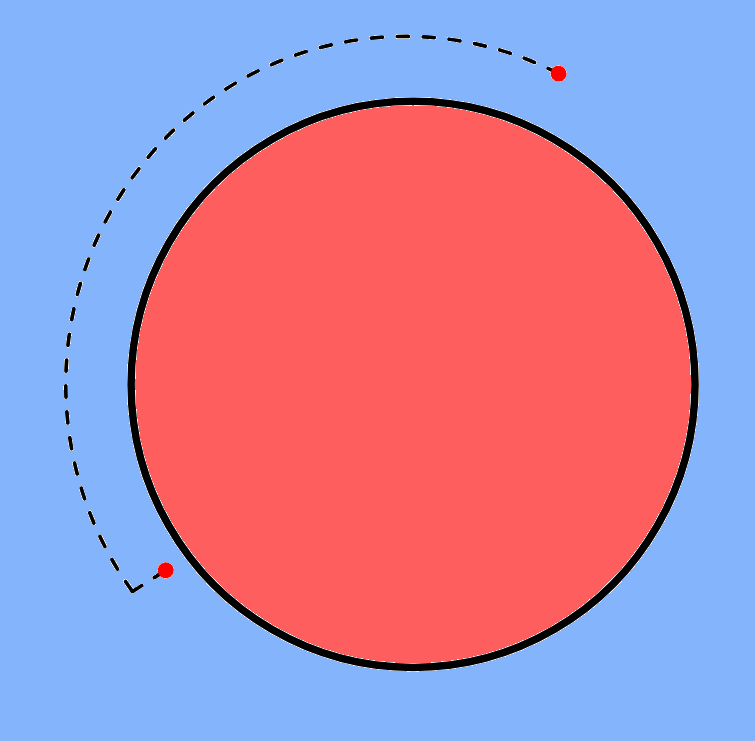
\includegraphics[width = 0.3\textwidth]{Chemin radial.png}
\end{figure}

On admettra également le résultat suivant (réf ici)

\begin{tcolorbox}[colback = purple!20!white, colframe = purple!60!white, title = Théorème 1]
    Soient $x \neq y \in \mathbb{R}^2$ et $c$ un chemin de $x$ à $y$\\
    Il existe un chemin $d$ injectif de $x$ à $y$ tel que $d \subset c$
\end{tcolorbox}

\section{Etude des lacets à retours finis}

On formalise enfin l'intution qu'on a en tracant le lacet\\
On se fixe dans cette partie $\gamma$ un lacet à retours finis

\subsection{Définitions}

\begin{tcolorbox}[colback = yellow!60!white, colframe = orange!90!white, title = Définition 4]
    On définit pour $t \in [0, 1]$ le nombre de sorties à l'instant $t$
    \[\forall x \in I_{\gamma}, S(x, t) = |\gamma^{-1}(\{x\}) \cap [0, t]|\]
    et, en notant $I_{\gamma}(t) = I_{\gamma} \cap \gamma([0, t])$
    \[r_{\gamma}(t) = \sum_{x \in I_{\gamma}(t)} S(x ,t) - 1\]
\end{tcolorbox}
\vspace{0.5cm}
Notons qu'il s'agit des définitions précedemment données, appliquées au chemin $\gamma_{\mid[0, t]}$ pour $t \in [0, 1]$
\vspace{0.5cm}
\begin{tcolorbox}[colback = yellow!60!white, colframe = orange!90!white, title = Définition 5]
    Soit $t \in [0, 1]$\\
    On note $C_{\gamma}(t)$ l'ensemble des composantes connexes par arcs de
    $\mathbb{R}^2 \backslash \gamma([0, t])$
\end{tcolorbox}

\vspace{0.5cm}
On a donc par cette définition que $|C_{\gamma}(1)|$ correspond à l'ensemble des composantes connexes par arc du
complémentaire de $\gamma$ dans le plan

\subsection{Subdivision minimale}

On montre ici une propriété essentielle à la formalisation de notre intuition concernant le tracé des lacets à retours finis
\\~\\
\begin{tcolorbox}[colback=purple!20!white, colframe=purple!60!white, title = Proposition 9]
    $r_{\gamma}$ est une fonction en escalier. De plus, la subdivision minimale
    associée à $r_{\gamma}$, $(t_n)_{0 \leq n \leq r(\gamma)}$ vérifie
    \[\forall n \in \llbracket 0, r(\gamma) -1 \rrbracket, r_{\gamma}(t_{n+1}) = 1 + r_{\gamma}(t_n)\]
    et
    \[ \forall n \in \llbracket 1, r(\gamma) \rrbracket, \gamma(t_n) \in I_{\gamma}(t_n) \]
\end{tcolorbox}
\vspace{0.5cm}

\begin{proof}
Notons que pour tout $x \in I_{\gamma}$, $t \longmapsto S(x, t)$ est croissante\\
Donc $r_{\gamma}$ est croissante\\
De plus elle ne prend que des valeurs entières et est bornée, elle est alors en escalier
\\~\\
Supposons qu'elle ne le soit pas, alors pour toute subdivision $(t_n)_{0 \leq n \leq p}$ de $[0, 1]$, il existe
$n \in \llbracket 0, p-1 \rrbracket$ tel que $r_{\gamma}$ ne soit pas constante sur $]t_n, t_{n+1}[$\\
Montrons par récurrence que pour tout $k \in \mathbb{N}^*$, $r_{\gamma}$ prend $k$ valeurs distinctes\\
C'est évident pour $k = 1$\\
Supposons la propriété vraie au rang $k \in \mathbb{N}$\\
Notons $v_0 < ... < v_{k-1} \in \mathbb{N}$ les $k$ premières valeurs prises par $r_{\gamma}$ (bien défini car $r_{\gamma}$
est à valeurs entières)\\
On pose alors $(t_n)_{0 \leq n \leq k}$ telle que
\[ \forall n \in \llbracket 0, k-1 \rrbracket, t_n = \inf \{ t \in [0, 1] \mid r_{\gamma}(t) = v_n\} \]
et $t_k = 1$
\\~\\
Comme $r_{\gamma}$ est croissante on a $t_0 \leq t_1 < ... < t_k$ (on peut si $t_0 = t_1$ remplacer la subdivision en n'en gardant qu'un)\\
On a alors, par croissance que $r_{\gamma}$ est constante sur les $]t_n, t_{n+1}[$ pour
$n \in \llbracket 0, k-2 \rrbracket$, en effet si elle y prenait d'autres valeurs, il s'agirait nécessairement par
définition des $(t_n)$ d'une valeur strictement supérieure à $v_{k-1}$, mais cela contredirait la croissance\\
On a de plus $r_{\gamma}(t_0) \leq r_{\gamma}(t_1) < r_{\gamma}(t_2) < ... < r_{\gamma}(t_{k-1}) < r_{\gamma}(t_k)$ :\\
Les inégalités strictes de $1$ à $k-1$ viennent de la définition des $(t_n)$ comme borne inférieure et de la croissance de $r_{\gamma}$\\
La dernière inégalité stricte vient du fait que $r_{\gamma}$ est nécessairement non constante sur $]t_{k-1}, t_k[$ par ce qui précède\\
Donc $r_{\gamma}$ prend $k$ valeurs distinctes
\\~\\
On a bien montré la propriété par récurrence\\
Mais alors, comme ces valeurs sont entières, $r_{\gamma}$ est non bornée, absurde
\\~\\
Considérons alors $(t_n)_{0 \leq n \leq p}$ la subdivision minimale associée à $r_{\gamma}$\\
Montrons d'abord que

\begin{equation}
    \forall n \in \llbracket 0, p \rrbracket, \forall t < t_n, r_{\gamma}(t) < r_{\gamma}(t_n)
\end{equation}
Supposons que non\\
Donc il existe $n \in \llbracket 0, p \rrbracket$ et $t < t_n$ tel que $r_{\gamma}(t_n) \leq r_{\gamma}(t)$\\
Comme $r_{\gamma}$ est croissante on a
\[\forall t' \in [t, t_n[, r_{\gamma}(t') = r_{\gamma}(t_n)\]
Puis on utilise la minimalité de $(t_n)$ :\\
- Si $n = p$, c'est absurde car $r_{\gamma}(t) < r(\gamma)$ pour $t \in [0, 1[$\\
- Sinon, alors par minimalité, $r_{\gamma}$ doit prendre une valeur strictement plus grande
que $r_{\gamma}(t_n)$ sur $]t_n, t_{n+1}[$\\
Donc pour tout $\varepsilon > 0$, $r_{\gamma}(t_n + \varepsilon) > r_{\gamma}(t_n)$, donc
par définition de $r_{\gamma}$, pour tout $\varepsilon > 0$, il existe $x \in I_{\gamma}
\cap \gamma(]t_n, t_n + \varepsilon[)$ tel que $S(x, t_n + \varepsilon) > 2$\\
On a donc trouvé une infinité d'intersections, absurde car $\gamma$ est à retours finis\\
On a bien la propriété annoncée\\
Cela implique en particulier que $r_{\gamma}$ est constante sur les $[t_n, t_{n+1}[$
\\~\\
Montrons ensuite qu'il existe $t \in [t_n, t_{n+1}[$ tel que
\[ \sum_{x \in I_{\gamma}(t_{n+1}) \backslash \gamma([0, t])} S(x, t_{n+1}) - 1 = 0\]
Il suffit de remarquer que $I_{\gamma}(t_{n+1})$ étant fini, il existe $t \in [t_n, t_{n+1}[$ tel que
$|I_{\gamma}(t_{n+1}) \backslash \gamma([0, t])| \leq 1$\\
Si l'ensemble est vide, c'est terminé\\
Sinon, $\gamma(t_{n+1}) \notin \gamma([0, t_{n+1}[)$, donc $S(\gamma(t_{n+1}, t_{n+1})) = 1$\\
Donc la somme vaut bien 0
\\~\\
Enfin, on considère un tel $t \in [t_n, t_{n+1}[$\\
On a donc d'après ce qui précède
\[ r_{\gamma}(t_{n+1}) - r_{\gamma}(t) = \sum_{x \in I_{\gamma}(t)} S(x, t_{n+1}) - S(x, t) \geq 1\]
Il existe donc un $x \in I_{\gamma}(t)$ tel que $S(x, t_{n+1}) > S(x, t)$\\
Par minimalité de la subdivision, on a que $S(x, t') = S(x, t)$ pour $t \leq t' < t_{n+1}$
( le cas contraire le nombre de retours aurait augmenté entre $t_n$ et $t_{n+1}$ )\\
Donc nécessairement $x = \gamma(t_{n+1})$, ce qui montre que ce $x$ est unique\\
De plus il vient que
\[ | \gamma^{-1} \{ x \} \cap [0, t_{n+1}] | = 1 + | \gamma^{-1} \{ x \} \cap [0, t_{n+1}[ |\]
Donc
\[ \forall t' \in [t, t_{n+1}[, S(x, t_{n+1}) = 1 + S(x, t')\]
Donc comme ce $x$ est unique, on a
\[ \forall t' \in [t, t_{n+1}[, r_{\gamma}(t_{n+1}) = 1 + r_{\gamma}(t)\]
Or $r_{\gamma}$ est constante sur $[t_n, t_{n+1}[$ par les résultats précédents on a 
$r_{\gamma}(t_{n+1}) = 1 + r_{\gamma}(t_n)$\\
Puisque $r_{\gamma}$ prends des valeurs de $r_{\gamma}(0) = 0$ à $r_{\gamma}(t_p) = r(\gamma)$,
on en déduit que $p = r(\gamma)$\\

\end{proof}

\begin{tcolorbox}[colback=purple!20!white, colframe=purple!60!white, title = Corollaire 1]
    Pour tout $n \in \llbracket 0, r(\gamma)-1 \rrbracket$, $\gamma(]t_n, t_{n+1}[)$ ne rencontre pas
    $\gamma([0, t_n])$
\end{tcolorbox}

\begin{proof}
    Soit $t \in ]t_n, t_{n+1}[$\\
    Supposons par l'absurde que $\gamma(t) \in \gamma([0, t_n])$\\
    Alors $S(\gamma(t), t_{n+1}) - S(\gamma(t), t_n) \geq 1$, et par la Proposition 9, comme $\gamma(t_{n+1}) \in I_{\gamma}(t_{n+1})$,
    $S(\gamma(t_{n+1}), t_{n+1}) \geq 2$, donc
    $r_{\gamma}(t_{n+1}) \geq 2 + r_{\gamma}(t_n)$, absurde\\
\end{proof}

\begin{tcolorbox}[colback=purple!20!white, colframe=purple!60!white, title = Corollaire 2]
    Pour tout $n \in \llbracket 0, r(\gamma)-1 \rrbracket$, $\gamma$ est injective sur $]t_n, t_{n+1}[$
\end{tcolorbox}

\begin{proof}
    Soit $x \in \gamma$\\
    Supposons par l'absurde qu'il existe $t_1 \neq t_2 \in ]t_n, t_{n+1}[$ tels que $x = \gamma(t_1) = \gamma(t_2)$\\
    Donc $S(x, t_{n+1}) \geq 2$ et par la Proposition 9, $S(\gamma(t_{n+1}), t_{n+1}) \geq 2$\\
    Au total on a $r_{\gamma}(t_{n+1}) \geq 2 + r_{\gamma}(t_n)$, absurde
\end{proof}

\subsection{Résultats sur $C_{\gamma}$}

\begin{tcolorbox}[colback=purple!20!white, colframe=purple!60!white, title = Proposition 10]
    Soit $t \in [0, 1]$, et $V$ un ouvert de $\mathbb{R}^2 \backslash \gamma([0, t])$, connexe par arcs\\
    On a
    \[V \in C_{\gamma}(t) \Longleftrightarrow \operatorname{Fr}(U) \subset \gamma([0, t])\]
\end{tcolorbox}

\begin{proof}
Sens direct :\\
On a, comme $\gamma([0, t])$ est fermé par continuité :
\begin{align*}
    \operatorname{Fr}(\mathbb{R}^2 \backslash \gamma([0, t])) &= \overline{\mathbb{R}^2 \backslash \gamma([0, t])} \cap \gamma([0, t])\\
    &\subset \gamma([0, t])
\end{align*}
Puis par la Proposition 3, on pour $V \in C_{\gamma}(t)$, comme $\gamma([0, t])$ est fermé,
$\operatorname{Fr}(V) \subset \operatorname{Fr}(\mathbb{R}^2 \backslash \gamma([0, t])) \subset \gamma([0, t])$
\\~\\
Sens réciproque :\\
On raisonne par contraposée
\\~\\
Si $V \notin C_{\gamma}(t)$\\
Comme $V \subset \mathbb{R}^2 \backslash \gamma([0, t])$, il existe $U \in C_{\gamma}(t)$
tel que $V \cap U \neq \varnothing$\\
Donc $V \subsetneq U$ par la Proposition 4, et donc $U$ rencontre $V$ et son complémentaire\\
Donc par connexité par arcs et la Proposition 1 de $U$, $U \cap \operatorname{Fr}(V) \neq \varnothing$, et donc
$\operatorname{Fr}(V) \nsubseteq \gamma([0, t])$ car $U \cap \gamma([0, t]) = \varnothing$

\end{proof}

\begin{tcolorbox}[colback = purple!20!white, colframe = purple!60!white, title = Proposition 11]
    Pour tout $t \in [0, 1]$, il n'existe qu'un seul $V \in C_{\gamma}(t)$ non borné
\end{tcolorbox}

\begin{proof}
    Comme $[0, t]$ est compact et $\gamma$ continue, $\gamma([0, t])$ est borné\\
    Soit $r > 0$ tel que $\gamma([0, t]) \subset \mathcal{B}(0, r)$\\
    $\mathbb{R}^2 \backslash \mathcal{B}(0, r)$ est ainsi une partie connexe non bornée de 
    $\mathbb{R}^2 \backslash \gamma$\\
    Donc il existe $V \in C_{\gamma}(t)$ contenant cet ensemble, et donc non borné
    \\~\\
    Soit $U \in C_{\gamma}(t)$ non bornée\\
    $U$ rencontre alors $\mathbb{R}^2 \backslash \mathcal{B}(0, r)$, donc $U \cap V \neq \varnothing$, 
    donc $U = V$\\
    On a bien l'unicité
\end{proof}

\vspace*{0.5cm}

On se fixe pour les trois prochains lemmes $a, b \in [0, 1]$ tels que $a < b$, et on suppose qu'il existe $V \in C_{\gamma}(a)$ tel que
$\gamma(]a, b[) \subset V$

\begin{tcolorbox}[colback = purple!20!white, colframe = purple!60!white, title = Lemme de préservation]
    Les composantes connexes par arcs du complémentaire dans le plan de $\gamma([0, a])$ distinctes de $V$,
    sont également des composantes connexes par arcs du compléementaire de $\gamma([0, b])$, et réciproquement. En d'autres termes
    \[ C_{\gamma}(a) \cap C_{\gamma}(b) = C_{\gamma}(a) \backslash \{V \}\]
\end{tcolorbox}

\begin{proof}
    Montrons d'abord que $C_{\gamma}(a) \backslash \{ V \} \subset C_{\gamma}(b) \cap C_{\gamma}(a)$
    \\~\\
    Notons d'abord que $\gamma(b) \in \overline{V}$ : en effet par continuité, on a
    $\gamma(b) = \lim_{t \rightarrow b^-} \gamma(t)$\\
    Soit $U \in C_{\gamma}(a) \backslash \{ V \}$\\
    On a $\overline{V} \cap U = \varnothing$ : si ce n'était pas le cas, il existerait un point de $\overline{V}$
    dans $U$. Comme $U$ est ouvert, il est voisinage de ce point, or tout voisinage de ce point rencontre $U$\\
    Or $V \cap U = \varnothing$ et donc $\overline{V} \cap U = \varnothing$
    \\~\\
    Enfin, $U$ est connexe par arcs, $\operatorname{Fr}(U) \subset \gamma([0, b])$, et
    \[ \gamma([0, b]) \cap U = (\gamma([0, a]) \cap U) \cup (\gamma(]a, b]) \cap U) = \varnothing\]
    car $\gamma(]a, b]) \subset \overline{V}$\\
    Par la Proposition 10, $U \in C_{\gamma}(b)$, donc $C_{\gamma}(a) \backslash \{ V \} \subset C_{\gamma}(b) \cap C_{\gamma}(a)$
    \\~\\
    Réciproquement, si $U \in C_{\gamma}(a) \cap C_{\gamma}(b)$, alors $U \neq V$ :\\
    En effet, $V \notin C_{\gamma}(b)$ car $V \cap \gamma(]a, b[) \neq \varnothing$\\
    On a bien $C_{\gamma}(a) \cap C_{\gamma}(b) = C_{\gamma}(a) \backslash \{ V \}$
\end{proof}

\begin{tcolorbox}[colback = purple!20!white, colframe = purple!60!white, title = Lemme 1]
    Soit $\gamma$ un lacet à retours finis, et $a < b \in [0, 1]$\\
    On suppose qu'il existe $V \in C_{\gamma}(a)$ tel que $\gamma(]a, b[) \subset V$ et $\gamma(b) \notin V$\\
    Pour tout $U \in C_{\gamma}(b) \backslash C_{\gamma}(a)$, on a
    \[ \operatorname{Fr}(U) \cap \gamma(]a, b[) \neq \varnothing\]
\end{tcolorbox}

\begin{proof}
    Supposons par l'absurde que $\operatorname{Fr}(U) \cap \gamma(]a, b[) = \varnothing$\\
    $\gamma(b)$ est l'unique point de $\operatorname{Fr}(U)$ dans $\gamma(]a, b])$\\
    Comme $\gamma(]a, b[) \subset V$ et par continuité de $\gamma$, $\gamma(b) \in \operatorname{Fr}(V)$\\
    Par la Proposition 10, $\gamma(b) \in \gamma([0, a])$
    \\~\\
    Par cette même propriété, $\operatorname{Fr}(U) \subset \gamma([0, b])$\\
    Or par hypothèse et ce qui précède, on a donc $\operatorname{Fr}(U) \subset \gamma([0, a])$\\
    Donc, comme $U$ est connexe et $U \cap \gamma([0, a]) \subset U \cap \gamma([0, b]) = \varnothing$, on a $U \in C_{\gamma}(a)$\\
    Absurde
\end{proof}

\begin{tcolorbox}[colback = purple!20!white, colframe = purple!60!white, title = Lemme d'apparition]
    Soit $\gamma$ un lacet à retours finis, et $a < b \in [0, 1]$\\
    On suppose qu'il existe $V \in C_{\gamma}(a)$ tel que $\gamma(]a, b[) \subset V$\\
    Notons $\mathcal{C}$ l'ensemble des composantes connexes par arc de $V \backslash \gamma([a, b])$\\
    On a
    \[ C_{\gamma}(b) \backslash C_{\gamma}(a) = \mathcal{C}\]
\end{tcolorbox}

\begin{proof}
    Montrons d'abord $C_{\gamma}(b) \backslash C_{\gamma}(a) \subset \mathcal{C}$
    \\~\\
    Soit $U \in C_{\gamma}(b) \backslash C_{\gamma}(a)$\\
    Donc par la Proposition 10, $\operatorname{Fr}(U) \cap \gamma(]a, b]) \neq \varnothing$\\
    Si $\gamma(b) \in V$, alors $\overline{U} \cap V \neq \varnothing$\\
    Si $\gamma(b) \notin V$, $\operatorname{Fr}(U) \cap \gamma(]a, b[) \neq \varnothing$ par le Lemme 1
    \\~\\
    Donc au total $\overline{U} \cap V \neq \varnothing$\\
    Comme $V$ est un voisinage de tout ses points, et que tout voisinage d'un point de $\overline{U}$ rencontre $U$, on a
    $U \cap V \neq \varnothing$\\
    Donc $U \subset V$ par la Proposition 4, car $U \in C_{\gamma}(b)$
    \\~\\
    Donc $U \subset V \backslash \gamma([a, b])$ car $U \cap \gamma([a, b]) = \varnothing$\\
    Comme $U$ est connexe par arcs, par la Proposition 4 il existe $U' \in \mathcal{C}$ tel que $U \subset U'$\\
    Si $U' \backslash U \neq \varnothing$ par la Proposition 1, par connexité de $U'$, $U'$ rencontre $\operatorname{Fr}(U)$ donc
    $\gamma([0, b])$\\
    Or $U' \subset V \backslash \gamma([a, b])$ et $V \cap \gamma([0, a]) = \varnothing$, donc c'est absurde\\
    Donc $U' = U$\\
    On a bien $C_{\gamma}(b) \backslash C_{\gamma}(a) \subset \mathcal{C}$
    \\~\\
    Réciproquement, soit $U \in \mathcal{C}$\\
    Donc $U$ est connexe par arcs, $U \subset V \backslash \gamma([a, b]) \subset \mathbb{R}^2 \backslash \gamma([0, b])$, et
    Montrons que $\operatorname{Fr}(U) \subset \gamma([0, b])$\\
    On a d'abord
    \begin{align*}
        \operatorname{Fr}(V \backslash \gamma([a, b])) &= \overline{V \backslash \gamma([a, b])} \backslash (V \backslash \gamma([a, b]))\\
        &= \overline{V \backslash \gamma([a, b])} \cap (\mathbb{R}^2 \backslash V \cup \gamma([a, b]))\\
        &\subset (\operatorname{Fr}(V) \cap \overline{\mathbb{R}^2 \backslash \gamma([a, b])})
        \cup (\gamma([a, b]) \cap \overline{V \backslash \gamma([a, b])}\\
        &\subset \gamma([0, b])
    \end{align*}
    Puis, par la Proposition 3, on a $\operatorname{Fr}(U) \subset \operatorname{Fr}(V \backslash \gamma([a, b]))$\\
    Donc $\operatorname{Fr}(U) \subset \gamma([0, b])$\\
    Donc $U \in C_{\gamma}(b)$ par la Proposition 10\\
    Puis, $U \notin C_{\gamma}(a)$, car $U \subsetneq V$ et $V \in C_{\gamma}(a)$\\
    Donc $U \in C_{\gamma}(b) \backslash C_{\gamma}(a)$
    \\~\\
    On a bien $\mathcal{C} = C_{\gamma}(a) \backslash C_{\gamma}(b)$
\end{proof}
\vspace*{0.5cm}
On montre ensuite que dans le cas de la subdivision minimale, un tel $V$ existe toujours
\\~\\

\begin{tcolorbox}[colback = purple!20!white, colframe = purple!60!white, title = Proposition 12]
    Soit $\gamma$ un lacet à retours finis et $(t_n)$ la subdivision minimale associée à $r_{\gamma}$\\
    Soit $n \in \llbracket 0, r(\gamma)-1 \rrbracket$\\
    Il existe $V \in C_{\gamma}(t_n)$ tel que $\gamma(]t_n, t_{n+1}[) \subset V$
\end{tcolorbox}

\begin{proof}
    Comme $C_{\gamma}(t_n)$ est l'ensemble des composantes connexes par arcs délimitées par $\gamma([0, t_n])$ on a
    \[ \bigcup_{V \in C_{\gamma}(t_n)} V = \mathbb{R}^2 \backslash \gamma([0, t_n]) \]
    
    Donc par ce qui précède il existe $V \in C_{\gamma}(t_n)$ tel que $\gamma(t) \in V$
    \\~\\
    Donc $\gamma(]t_n, t_{n+1}[)$ est connexe par arcs, et rencontre $V \in C_{\gamma}(t_n)$\\
    De plus $\gamma(]t_n, t_{n+1}[) \cap \gamma([0, t_n]) = \varnothing$ par ce qui précède\\
    Donc par la Proposition 4, on a $\gamma(]t_n, t_{n+1}[) \subset V$
\end{proof}

\begin{tcolorbox}[colback = purple!20!white, colframe = purple!60!white, title = Lemme 2]
    Soit $\gamma$ un lacet à retours finis et $t \in [0, 1]$\\
    Soit $V \in C_{\gamma}(t)$ et $x \in \operatorname{Fr}(V)$\\
    Alors il existe $r > 0$ tel que pour tout $\varepsilon \in ]0, r[$, $\mathcal{B}(x, \varepsilon) \cap V$
    a un nombre fini de composantes connexes par arc
\end{tcolorbox}

\begin{proof}
    Si $t = 0$, on a la propriété
    \\~\\
    Sinon, on se donne d'abord comme $\gamma$ est à retours finis $r > 0$ tel que $I_{\gamma} \cap \mathcal{B}(x, r) \subset
    \{ x \}$ et tel que $\gamma([0, t]) \backslash \mathcal{B}(x, r) \neq \varnothing$
    \\~\\
    Supposons à présent par l'absurde que pour tout $r > 0$ il existe $\varepsilon \in ]0, r[$ tel que
    $\mathcal{B}(x, \varepsilon) \cap V$ ait une infinité de composantes connexes par arcs\\
    Comme $\operatorname{Fr}(V) \subset \gamma([0, t])$, on choisit $c \in [0, t]$ tel que $\gamma(c) = x$\\
    Puis on pose
    \[ a_0 = \inf\{ t' \in [0, 1] \mid \gamma([t', c]) \subset \mathcal{B}(x, r) \} \text{ et }
    b_0 = \sup\{ t' \in [0, 1] \mid \gamma([c, t']) \subset \mathcal{B}(x, r) \} \]
    Comme $\gamma([0, t]) \backslash \mathcal{B}(x, r) \neq \varnothing$, on a $[a_0, b_0] \neq [0, t]$\\

\end{proof}

\section{Le théorème}

Nous avons à présent tout les outils pour démontrer le théorème

\subsection{Les cas d'augmentation}

On se fixe $\gamma$ un lacet à retours finis\\
On se donne $(t_n)$ la subdivision minimale adaptée à $r_{\gamma}$\\
On distingue 2 cas d'augmentation du nombre de retours de $t_n$ à $t_{n+1}$ de la subdivision minimale
\\~\\

Dans le premier cas, le lacet "traverse" une composante connexe par arcs déjà présente\\
Dans le second, le lacet forme une boucle à l'intérieur d'une autre composante connexe par arcs\\
Ils sont ici représentés par des composantes bornées, mais cette disjonction s'applique aussi lorsque le lacet traverse une composante
non bornée
\\~\\
Plus formellement, pour $n \in \llbracket 0, r(\gamma) -1 \rrbracket$ on a :
\begin{itemize}
    \item Cas 1 : Soit $\gamma(t_{n+1}) \notin \gamma(]t_n, t_{n+1}[)$\\
    \item Cas 2 : Soit $\gamma(t_{n+1}) \in \gamma(]t_n, t_{n+1}[])$
\end{itemize}

\begin{figure}[h]
    \caption{Les différents cas}
    \centering
    \includegraphics*[width=0.4\textwidth]{Cas 1.png}
    \includegraphics*[width=0.4\textwidth]{Cas 2.png}
\end{figure}

\vspace*{3cm}

\subsection{La démonstration}

\begin{tcolorbox}[colback=purple!20!white, colframe=purple!60!white, title = Théorème des retours]
    Un lacet $\gamma$ à retours finis délimite $r(\gamma)$ composantes connexes par arcs bornées
\end{tcolorbox}

\begin{proof}
    Soit $\gamma$ un lacet à retours finis\\
    Montrons la propriété suivante par récurrence finie sur $n \in \llbracket 0, r(\gamma) \rrbracket$
    \[ \mathcal{H}(n) : r_{\gamma}(t_n) + 1 = |C_{\gamma}(t_n)| \]
    Le cas $n = 0$ est évident car $\mathbb{R}^2 \backslash \{ \gamma(0) \}$ est connexe par arcs et non borné
    \\~\\
    Supposons $\mathcal{H}(n)$ pour un $n \in \llbracket 0, r(\gamma)-1 \rrbracket$\\
    Notons $x = \gamma(t_n)$ et $y = \gamma(t_{n+1})$\\
    Par la Proposition 12, on se donne $V \in C_{\gamma}(t_n)$ tel que $\gamma(]t_n, t_{n+1}[) \subset V$
    \\~\\
    Montrons alors que $V \backslash \gamma([t_n, t_{n+1}])$ a exactement 2 composantes connexes par arc
    \begin{itemize}
        \item Cas 1 : Si $y \notin \gamma(]t_n, t_{n+1}[)$\\
        On a donc $y \in \gamma([0, t_n])$\\
        Il existe alors un chemin à retours finis de $y$ à $x$ dans $\gamma([0, t_n])$, obtenu en suivant le tracé du lacet\\
        On se donne alors $c$ un chemin injectif de $y$ à $x$ par la Proposition 6\\
        On construit alors une courbe de Jordan $\alpha$ en concaténant $c$ à $\gamma_{\mid [t_n, t_{n+1}]}$, par les Corollaires 1 et 2
        \\~\\
        Montrons que $V \cap U$ et $V \cap U'$ sont les composantes connexes par arcs de $V \backslash \gamma([t_n, t_{n+1}])$\\
        Montrons d'abord que $V \cap U$ est connexe par arcs
        \\~\\
        Pour cela, considérons $C_1$ et $C_2$ deux composantes connexes par arcs de $V \cap U$ et montrons qu'elles
        appartiennent à $C_{\gamma}(t_{n+1}) \backslash C_{\gamma}(t_n)$\\
        On mène pour cela une démonstration très similaire au Lemme d'apparition, en exploitant le fait que
        $\operatorname{Fr}(V \cap U) \cap V = \gamma(]t_n, t_{n+1}[)$ par construction
        \\~\\
        Par la Proposition 10, $\operatorname{Fr}(C_1) \cap \gamma(]t_n, t_{n+1}[) \neq \varnothing$ et de même pour $C_2$\\
        On se donne alors $t \leq t' \in ]t_n, t_{n+1}[$ tels que $\gamma(t)$ et $\gamma(t')$ appartiennent respectivement à ces
        intersections\\
        Comme $\gamma([t, t']) \subset V$ et est compact, on se donne $r > 0$ tel que pour tout point de $\gamma([t, t'])$,
        la boule centrée en ce point de rayon $r$ est incluse dans $V$\\
        Comme $\gamma(t)$ et $\gamma(t')$ sont des points frontière, il existe dans tout voisinage de ces points respectivement des
        points de $C_1$ ou $C_2$\\
        Par ce qui precède et la Proposition 7, il existe donc un chemin dans $V \cap U$ de $C_1$ à $C_2$ et donc $C_1 = C_2$\\
        $V \cap U$ est bien connexe par arcs et par le même raisonnement $V \cap U'$ également
        \\~\\
        Par la Proposition 5, comme ce sont des ouverts connexes par arc formant une partition de $V \backslash \gamma([t_n, t_{n+1}])$, il s'agit
        de ses composantes connexes par arc
        \\~\\
        \item Cas 2 : si $y \in \gamma(]t_n, t_{n+1}[)$\\
        On se donne $t' \in [t_n, t_{n+1}]$ tel que $\gamma(t') = y$\\
        Comme $\gamma_{\mid [t_n, t_{n+1}[}$ est injective par le Corollaire 2, $\gamma_{\mid [t', t_{n+1}]}$ est une courbe de Jordan\\
        On note $U$ sa composante bornée et $U'$ celle non bornée
        \\~\\
        Notons que dans ce cas, $n \neq r(\gamma)-1$ : en effet, si on avait $n = r(\gamma)$, alors $y = \gamma(0)$
        et donc $y \in \gamma([0, t_n])$, ce qui n'est pas le cas ici\\
        Il existe donc un chemin à retours finis $c$ de $y$ à $\gamma([0, t_n])$ exploitant le tracé du lacet à venir, soit
        $\gamma_{\mid [t_{n+1}, 1]}$
        \\~\\
        On se donne comme pour le cas 1, $C_1$ et $C_2$ des composantes connexes par arcs de $V \cap U'$,
        qui sont élements de $C_{\gamma}(t_{n+1})\backslash C_{\gamma}(t_n)$\\
        Leur frontières rencontrent donc $\gamma(]t_n, t_{n+1}])$ par la Proposition 10\\
        Soient $u \in \operatorname{Fr}(C_1) \cap \gamma(]t_n, t_{n+1}])$ et
        $v \in \operatorname{Fr}(C_2) \gamma(]t_n, t_{n+1}])$, distincts tout deux de $\gamma(t_{n+1})$\\
        De tels point existent car tout voisinage de $\gamma(t_{n+1})$ rencontre $U$ et $U'$ par construction\\
        Ainsi, si $\gamma(t_{n+1})$ était l'unique point de $\operatorname{Fr}(C_1) \cap \gamma(]t_n, t_{n+1}])$, comme une boule privée
        d'un point est connexe par arcs, alors on aurait $\operatorname{Fr}(C_1) \cap (V \cap U') \neq \varnothing$\\
        Or par la Proposition 3, $\operatorname{Fr}(C_1) \subset \operatorname{Fr}(V \cap U')$ et c'est donc absurde
        \\~\\ 
        On se donne $a \leq b \in ]t_n, t_{n+1}[$ tels que $\gamma(a) = u$ et $\gamma(b) = v$ sans perte de généralité\\
        Notons que le chemin obtenu en concaténant, $\gamma([b, t_{n+1}])$, $c$ et $\gamma([t_n, a])$ est à retours finis
        et rencontre $\gamma([a, b])$ un nombre fini de fois car $\gamma$ est à retours finis\\
        On se donne alors un nouveau chemin $d$ de $v$ à $u$ injectif, et ne rencontrant pas $\gamma([a, b])$ par les Propositions ? et 6\\
        On peut alors construire une courbe de Jordan exploitant $\gamma([a, b])$ et $d$\\
        Puis, on conclut comme dans le cas 1 que $C_1 = C_2$
        \\~\\
        Pour $V \cap U$, on procède de même manière que pour le cas 1, en utilisant la courbe de Jordan $\gamma_{\mid [t', t_{n+1}]}$
        \\~\\
        $V \cap U$ et $V \cap U'$ sont alors tout deux connexes par arcs, ouverts, et formant une partition de $V \backslash \gamma([t_n, t_{n+1}])$\\
        Par la Proposition 5
        \begin{figure}[h]
            \caption{Le chemin injectif de $y$ à $\gamma([0, t_n])$ dans $\gamma([t_{n+1}, 1])$, cas 2}
            \centering
            Le chemin est en gris.
            Les composantes connexes par arcs bornées des différentes courbes de Jordan construites sont en vert\\
            \includegraphics*[width = 0.5 \textwidth]{Unicité cas 2.png}
        \end{figure}
        \\~\\
    \end{itemize}
    Puis en utilisant les lemmes de préservation et d'apparition
    \begin{align*}
        |C_{\gamma}(t_{n+1})| &= |(C_{\gamma}(t_{n+1}) \backslash C_{\gamma}(t_n)) \sqcup (C_{\gamma}(t_{n+1}) \cap C_{\gamma}(t_n)) |\\
        &= 2 + |C_{\gamma}(t_n)| - 1\\
        &= r_{\gamma}(t_n) + 2\\
        &= r_{\gamma}(t_{n+1}) + 1
    \end{align*}
    \\~\\
    Au total par récurrence, on obtient $|C_{\gamma}(t_{r(\gamma)})| = |C_{\gamma}(1)| = r(\gamma) + 1$\\
    Par la Proposition 11, $\mathbb{R}^2 \backslash \gamma$ possède donc $r(\gamma)$ composantes connexes bornées

\end{proof}

\end{flushleft}
\end{document}